%%%%%%%%%%%%%%%%%%%%%%%%%%%%%%%%%%%%%%%%%%%%%%%%%%%%%%%%%%%%
% Document settings
\documentclass{ACGSeminar}

%%%%%%%%%%%%%%%%%%%%%%%%%%%%%%%%%%%%%%%%%%%%%%%%%%%%%%%%%%%%
% Own Packages

%%%%%%%%%%%%%%%%%%%%%%%%%%%%%%%%%%%%%%%%%%%%%%%%%%%%%%%%%%%%
% Own Definitions
\newcommand{\comment}[1]{}


%%%%%%%%%%%%%%%%%%%%%%%%%%%%%%%%%%%%%%%%%%%%%%%%%%%%%%%%%%%%
% BibTex
\bibliography{references}

%%%%%%%%%%%%%%%%%%%%%%%%%%%%%
% Hyphenations here
%%%%%%%%%%%%%%%%%%%%%%%%%%%%%
\hyphenation{Sa-tan-arch-aeo-li-deal-co-hell-ish}


%%%%%%%%%%%%%%%%%%%%%%%%%%%%%
% Title, Author, etc.

\begin{document}

\title{Re: Deep G-Buffers for Stable Global Illumination Approximation}

\author{Ferit Tohidi Far}

\maketitle

%%%%%%%%%%%%%%%%%%%%%%%%%%%%%%%%%%%%%%%%%%%%%%%%%%%%%%%%%%%%
% Abstract

\begin{abstract}%
G-buffers can be used to efficiently render images with large amounts of light sources. This is possible thanks to a process called "deferred rendering". Using 
g-buffers, we are only able to compute local illumination. By using deep g-buffers instead we can approximate global illumination, which is way more 
efficient than traditional global illumination methods like pathtracing, while of course not being physically accurate. We can make up for it, though, by also
approximating visual effects like ambient occlusion, color bleeding, reflections, depth of field and motion blur to create an acceptable result.
\end{abstract}

\keywords{nvidia, g-buffer, deep g-buffer, pathtracing, global illumination approximation, deferred shading, deferred rendering}
\tableofcontents

\label{cha:references}

\newpage

%%%%%%%%%%%%%%%%%%%%%%%%%%%%%%%%%%%%%%%%%%%%%%%%%%%%%%%%%%%%
% Introduction
\label{cha:introduction}
\section{Global illumination}
	Global illumination is a lighting effect that is achieved by not only computing direct light, but also indirect light, meaning that it is neccesary to take
	into account how light reflects and carries information (in the most basic case: color).
	\subsection{Physically correct methods}
	In order to generate physically correct images, which is a requirement for creating photorealistic images, we need to solve the rendering equation
	$$ L_o(\omega) = L_e(\omega) + \int_\Omega f(\omega, \omega')L_i(\omega')cos(n, \omega') \partial \omega' $$
	where 
	\begin{center}
		\begin{align*}
			&L_o(\omega) \text{ is the outgoing light in direction } \omega\text{,}\\
			&L_e(\omega) \text{ is the emmited light in direction } \omega\text{,}\\
			&f(\omega, \omega') \text{ is the BRDF\footnotemark} \text{,}\\
			&L_i(\omega') \text{ is the incoming light from direction } \omega'\\
			&\text{and } cos(n, \omega') \text{ is lambert reflectance\footnotemark}  \text{ .}
		\end{align*}
	\end{center}
	\addtocounter{footnote}{-1}
	\footnotetext{BRDF (Bidirectional random distribution function) basically returns the reflection/refraction direction of a ray on surface.}%
	\stepcounter{footnote}
	\footnotetext{Lambert reflectance describes the attentuation of light based on its incident angle to the surface.}%
	The most popular method for achieving this is pathtracing \cite{P2PATH}.
	\subsubsection{Pathtracing}
		Pathtracing solves the rendering equation by first sending camera rays through each individual pixel of the image plane and then tracing the ray back to the light source. If the lamp is hit the pixel gets painted painted with color, else black. Direct consequences of this are soft shadows and ambient occlusion. A maximum hop number caps the amount of times a ray is able to reflect. A hop number larger than 3 (3 in most cases, but it is dependent on the complexity of the scene) allows for global illumination. The reflections and refractions are essentially determined by the BRDF, which not only means that objects can be transparent, but we also get caustics\footnote{Caustics are areas with concentrated light. This happens due to light refracting.}. With each surface a ray hits it carries information from that surface, e.g. its color, and reflects it onto the next surface it hits. This causes color bleeding.
	\subsection{Computational difficulties of physically correct methods}
	Since we have to take into account every ray of light and its reflections, the computational difficulty becomes apparent \cite{DST}.
	% TODO insert time-complexity of pathtracing and time-complexity of deferred-rendering for comparison

\section{Deferred rendering}
	\subsection{How deferred rendering handles lighting more efficiently}
		The goal of deferred rendering is to postpone the shading stage. %TODO insert information about graphics pipeline of gpu
		Instead of shading right away, we compute necessary geometry buffers (g-buffers) and cache 
		them for later use. For all practical purposes, g-buffers have to at least consist of a frame-buffer, a normal-buffer and a z-buffer. Using only these g-buffers, 
		we can now compute the shading separately.
	\subsection{Deferred shading}

\section{Geometry-buffer (g-buffer)}
	Each geometry-buffer stores information of some sort for each individual pixel, meaning that they are all two-dimensional arrays.
	\subsection{Frame-buffer}%
		The frame-buffer stores color values.% 
		\begin{figure}[htb!]%
			\begin{center}%
				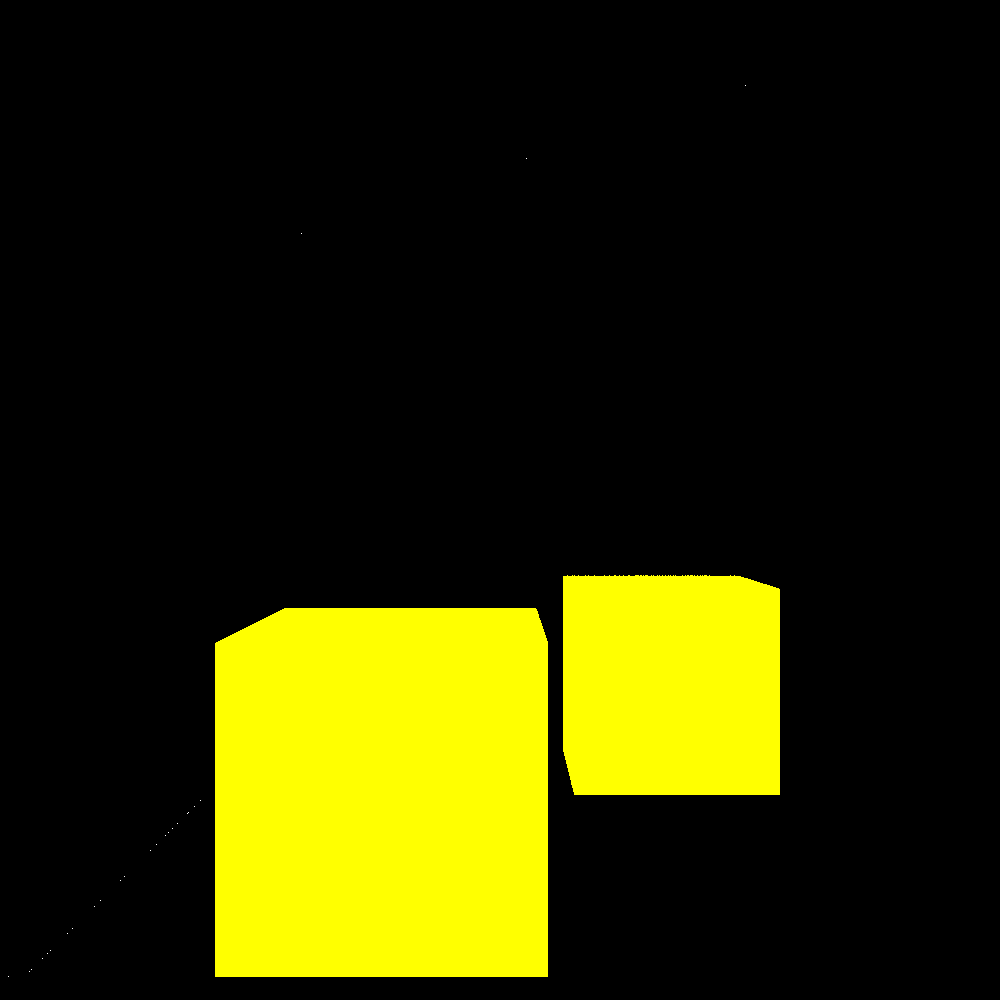
\includegraphics[width=7cm]{img/frame_buffer.png}
			\end{center}%
			\caption{Example of a frame-buffer (also called image-buffer). It shows a cornell box with white walls containing two blue cuboids.}%
			\label{fig:frame_buffer}%
		\end{figure}%
	\subsection{Z-buffer}
		The z-buffer stores depth values.
		\begin{figure}[htb!]%
			\begin{center}%
				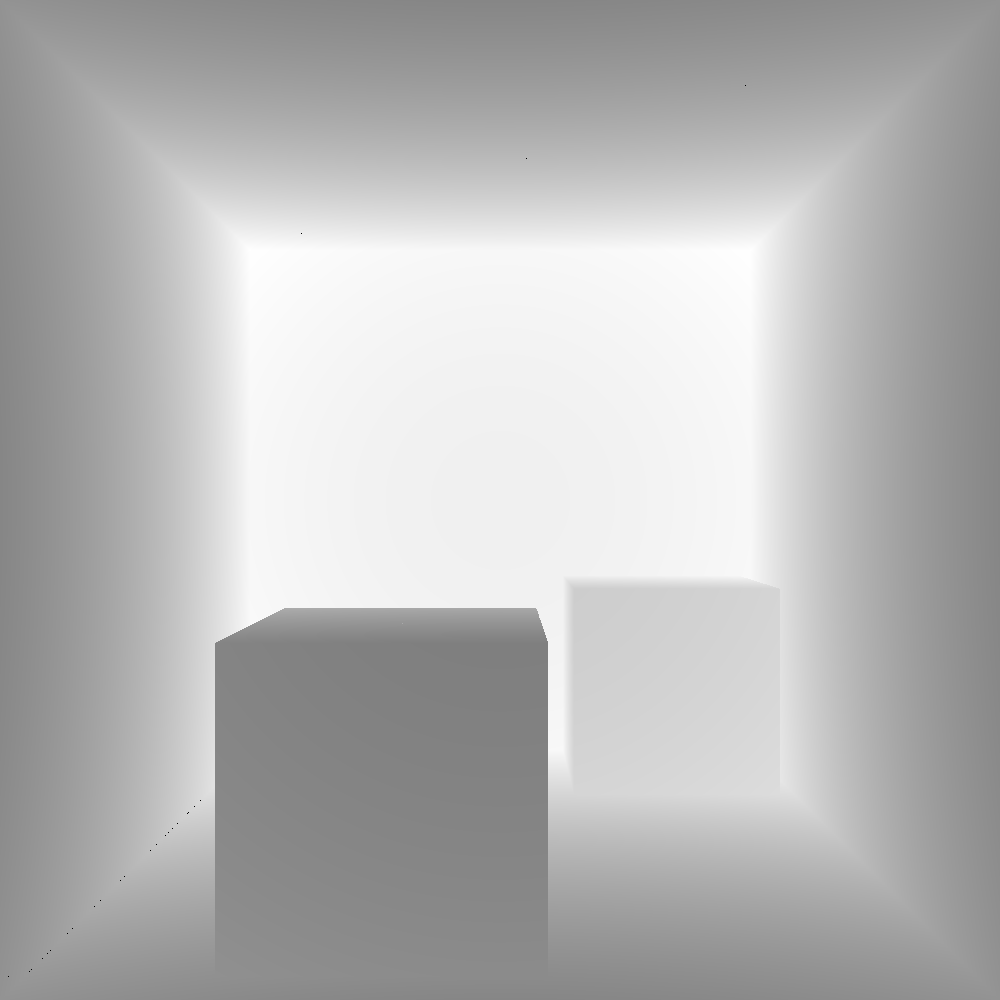
\includegraphics[width=7cm]{img/z_buffer.png}
			\end{center}%
			\caption{Example of a z-buffer. Since the z-buffer only stores distances as float values instead of actual colors they are interpreted as the grayscale value deduced by dividing each
			distance by the maximum distance from the cameras point of view.}%
			\label{fig:z_buffer}%
		\end{figure}%
	\subsection{Normal-buffer}
		The normal-buffer stores surface-normals.
		\begin{figure}[htb!]%
			\begin{center}%
				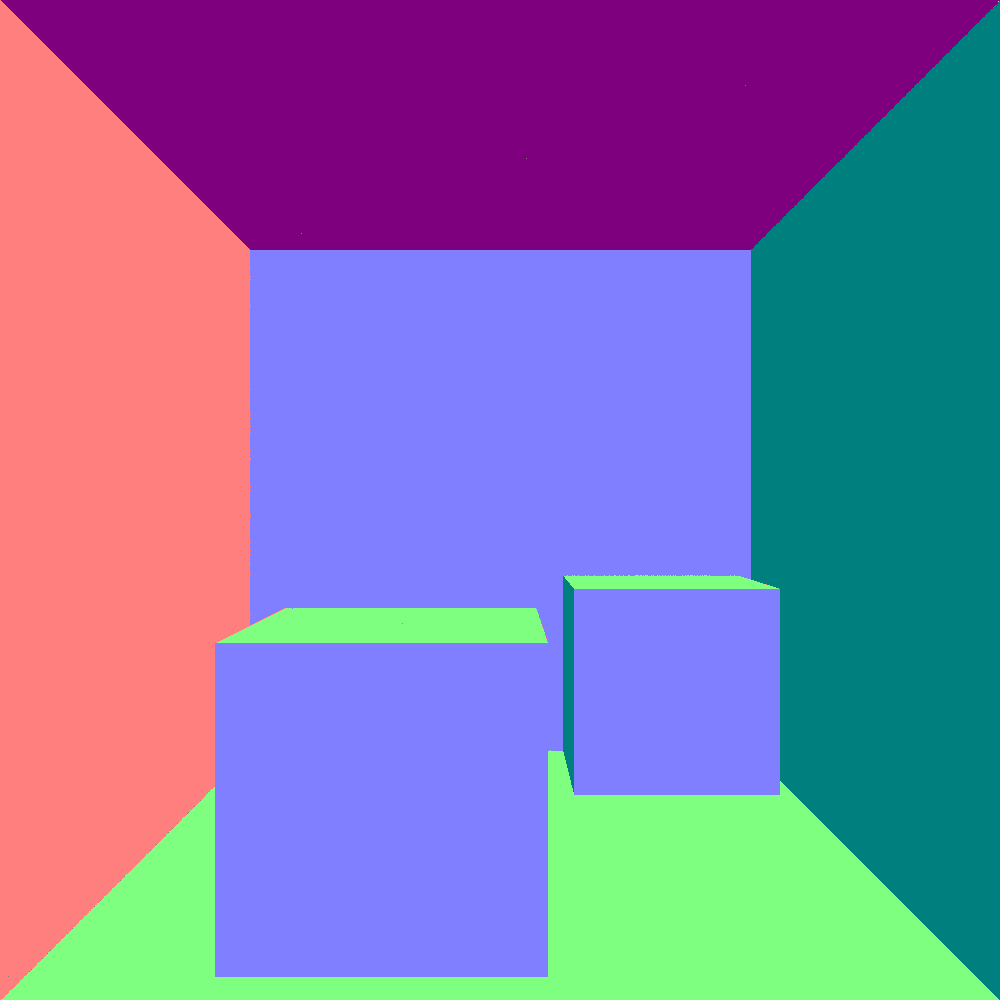
\includegraphics[width=7cm]{img/normal_buffer.png}
			\end{center}%
			\caption{Example of a normal-buffer. Normal vectors are usually normalized, meaning their values range from 0 to 1. Multiplying them with 255 gives us an RGB color. Since negative normals
			would cause negative RGB values we just take the absolute values.}%
			\label{fig:normal_buffer}%
		\end{figure}%
		Note that there are more possible buffers to choose from, but the three that were mentioned are the most essential in every g-buffer.
	\subsection{Computing local illumination using g-buffers}
		After having collected all our g-buffers we can now work on illumination. To do this we need to define some light sources. We distinguish between three types of light:
		Point-lights, spot-lights and directional-lights \cite{DST}. The simplest one is directional-light. We simply specify an origin in 3d space from which the light rays are sent. A point-light is a directional-light with a radius.

\section{Deep g-buffer}
	\subsection{Concept}
		Deep g-buffers use a concept similar to depth peeling. Instead of storing information about the closest surface, in an n layer deep g-buffer we also store information about the n-closest surface \cite{NDGB}.
	\subsection{How deep g-buffers approximate visual effects}


\section{Visual effects}
	The following are visual effects that are sought after, but some of them are hard or impossible to achieve physically correct without using
	computationally expensive methods. When using pathtracing, we get most of the following effects for free: 
	\subsection{Ambient occlusion}
		Ambient occlusion essentially describes how much shading the "in-betweens" of a 3d object gets. This effect can be efficiently approximated by using a method called - ironically - screen space ambient occlusion (SSAO). This method basically runs an edge detector over the z-buffer and paints those edges black. Since it only runs over the z-buffer it is considered screen space.
		%TODO insert graphics for AO here
	\subsection{Color bleeding}
		Color bleeding happens when light directs information from one hit-surface to another. Let A and B be objects. If A reflects light onto B and A's surface is blue, then B will also appear
		to be slightly blue on the reflected area. To have this happen it is obviously necessary to trace rays of some sort. This can be approximated, though, using ... %TODO how is this approximated?
		%TODO insert graphics for color bleeding here
	\subsection{Soft shadows}
		We can easily compute hard shadows using shadow mapping. This is done by projecting the scene from the light source's point of view and then projecting the scene from the camera's point of view while only actually painting the points with their respective colors if they are hit by light, else they are painted black. To get soft shadows, the points in shade simply get blended together with their surrounding points.
		%TODO insert graphics for soft and hard shadow
	\subsection{Transparency}
		A quick method to achieve transparency is depth peeling. \cite{NOIT}.

	\subsection{Reflection}
		Reflection ...

	\subsection{Depth of field}

	\subsection{Motion blur (in interactive applications)}

\section{Performance and output comparison}
	\subsection{Deep g-buffers vs pathtracing}

%%%%%%%%%%%%%%%%%%%%%%%%%%%%%%%%%%%%%%%%%%%%%%%%%%%%%%%%%%%%
% Bibliography
\printbibliography

\end{document}
